\documentclass[aspectratio=169]{../latex_main/tntbeamer}  % you can pass all options of the beamer class, e.g., 'handout' or 'aspectratio=43'
\usepackage{dsfont}
\usepackage{bm}
\usepackage[english]{babel}
\usepackage[T1]{fontenc}
%\usepackage[utf8]{inputenc}
\usepackage{graphicx}
\graphicspath{ {./figures/} }
\usepackage{algorithm}
\usepackage[ruled,vlined,algo2e,linesnumbered]{algorithm2e}
\usepackage{hyperref}
\usepackage{booktabs}
\usepackage{mathtools}

\usepackage{amsmath,amssymb}

\DeclareMathOperator*{\argmax}{arg\,max}
\DeclareMathOperator*{\argmin}{arg\,min}

\usepackage{amsbsy}
\newcommand{\vect}[1]{\bm{#1}}
%\newcommand{\vect}[1]{\boldsymbol{#1}}

\usepackage{pgfplots}
\pgfplotsset{compat=1.16}
\usepackage{tikz}
\usetikzlibrary{trees} 
\usetikzlibrary{shapes.geometric}
\usetikzlibrary{positioning,shapes,shadows,arrows,calc,mindmap}
\usetikzlibrary{positioning,fadings,through}
\usetikzlibrary{decorations.pathreplacing}
\usetikzlibrary{intersections}
\pgfdeclarelayer{background}
\pgfdeclarelayer{foreground}
\pgfsetlayers{background,main,foreground}
\tikzstyle{activity}=[rectangle, draw=black, rounded corners, text centered, text width=8em]
\tikzstyle{data}=[rectangle, draw=black, text centered, text width=8em]
\tikzstyle{myarrow}=[->, thick, draw=black]

% Define the layers to draw the diagram
\pgfdeclarelayer{background}
\pgfdeclarelayer{foreground}
\pgfsetlayers{background,main,foreground}

% Requires XeLaTeX or LuaLaTeX
%\usepackage{unicode-math}

\usepackage{fontspec}
%\setsansfont{Arial}
\setsansfont{RotisSansSerifStd}[ 
Path=../latex_main/fonts/,
Extension = .otf,
UprightFont = *-Regular,  % or *-Light
BoldFont = *-ExtraBold,  % or *-Bold
ItalicFont = *-Italic
]
\setmonofont{Cascadia Mono}[
Scale=0.8
]

% scale factor adapted; mathrm font added (Benjamin Spitschan @TNT, 2021-06-01)
%\setmathfont[Scale=1.05]{Libertinus Math}
%\setmathrm[Scale=1.05]{Libertinus Math}

% other available math fonts are (not exhaustive)
% Latin Modern Math
% XITS Math
% Libertinus Math
% Asana Math
% Fira Math
% TeX Gyre Pagella Math
% TeX Gyre Bonum Math
% TeX Gyre Schola Math
% TeX Gyre Termes Math

% Literature References
\newcommand{\lit}[2]{\href{#2}{\footnotesize\color{black!60}[#1]}}

%%% Beamer Customization
%----------------------------------------------------------------------
% (Don't) Show sections in frame header. Options: 'sections', 'sections light', empty
\setbeamertemplate{headline}{empty}

% Add header logo for normal frames
\setheaderimage{
	% 
\includegraphics[height=\logoheight]{figures/TNT_darkv4.pdf}
	
\includegraphics[height=\logoheight]{../latex_main/figures/luh_logo_rgb_0_80_155.pdf}
	% 
\includegraphics[height=\logoheight]{figures/logo_tntluh.pdf}
}

% Header logo for title page
\settitleheaderimage{
	% 
\includegraphics[height=\logoheight]{figures/TNT_darkv4.pdf}
	
\includegraphics[height=\logoheight]{../latex_main/figures/luh_logo_rgb_0_80_155.pdf}
	% 
\includegraphics[height=\logoheight]{figures/logo_tntluh.pdf}
}

% Title page: tntdefault 
\setbeamertemplate{title page}[tntdefault]  % or luhstyle
% Add optional title image here
%\addtitlepageimagedefault{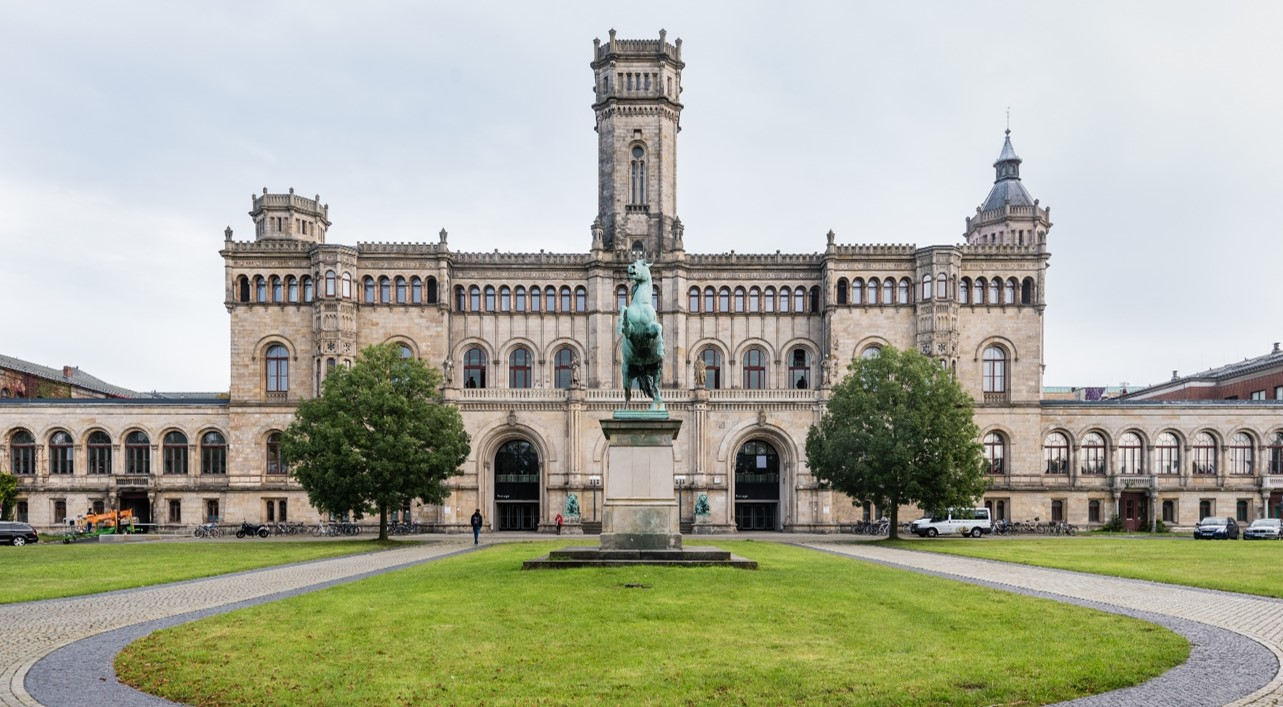
\includegraphics[width=0.65\textwidth]{figures/luh_default_presentation_title_image.jpg}}

% Title page: luhstyle
% \setbeamertemplate{title page}[luhstyle]
% % Add optional title image here
% \addtitlepageimage{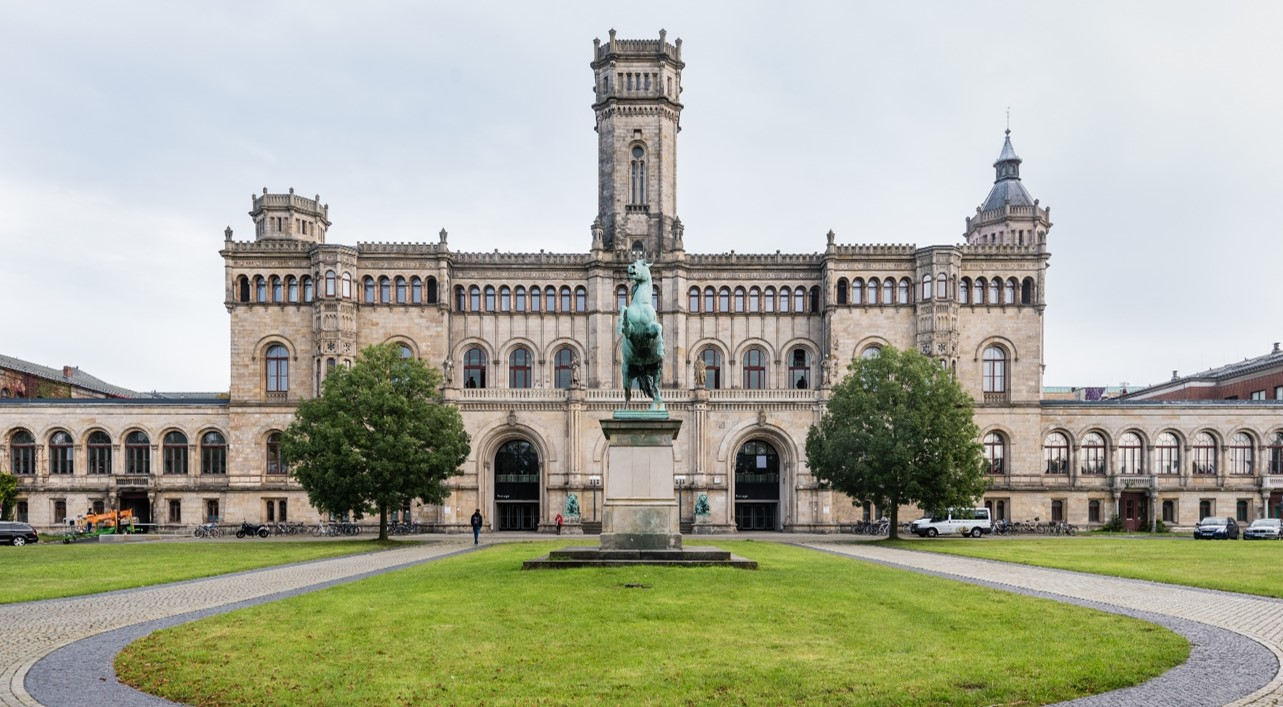
\includegraphics[width=0.75\textwidth]{figures/luh_default_presentation_title_image.jpg}}

\author[Abedjan \& Lindauer]{Ziawasch Abedjan \& Marius Lindauer\\[1em]
	
\includegraphics[height=\logoheight]{../latex_main/figures/luh_logo_rgb_0_80_155.pdf}\qquad
	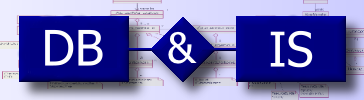
\includegraphics[height=\logoheight]{../latex_main/figures/DBIS_Kurzlogo.png}\qquad

\includegraphics[height=\logoheight]{../latex_main/figures/TNT_darkv4}\qquad

\includegraphics[height=\logoheight]{../latex_main/figures/L3S.jpg}	}
\date{Summer Term 2022; \hspace{0.5em} {
\includegraphics[height=1.5em]{../latex_main/figures/Cc-by-nc-sa_icon.svg.png}}; based on \href{https://ds100.org/fa21/}{[DS100]}
}


%%% Custom Packages
%----------------------------------------------------------------------
% Create dummy content
\usepackage{blindtext}

% Adds a frame with the current page layout. Just call \layout inside of a frame.
\usepackage{layout}


%%% Macros
%\renewcommand{\vec}[1]{\mathbf{#1}}
% \usepackage{bm}
%\let\vecb\bm

\title[Introduction]{DS: Introduction to Modeling}
\subtitle{What is a model?}

\graphicspath{ {./figure/} }
%\institute{}


\begin{document}
	
	\maketitle
	\begin{frame}{Data science lifecycle}
	    \begin{center}
	        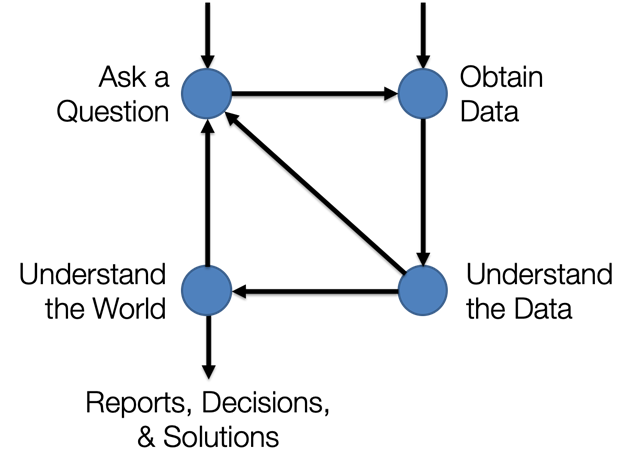
\includegraphics[scale=.65]{Bild1}
	    \end{center}
	    
	    We’re now moving to the fourth stage of the data science lifecycle – Understand the World – where we build models that try and generalize patterns in the data we collected.
	\end{frame}
	
	
	\begin{frame}{What is a model?}
	    \begin{columns}
	        \begin{column}{.5\textwidth}
	                %\begin{center}
	                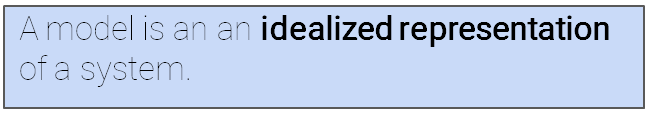
\includegraphics[scale=.4]{Bild3}\\
	                For example, we model the fall of an object on Earth as subject to a constant acceleration of 9.81 m/$s^2$ due to gravity.

	                \begin{itemize}
	                    \item While this describes the behavior of our system, it is merely an approximation.
	                    \item It doesn’t account for the effects of air resistance, local variations in gravity, etc.
	                    \item But in practice, it’s accurate enough to be useful!
	                \end{itemize}
	                %\end{center}
	                
	        \end{column}
	        
	        
	        \begin{column}{.5\textwidth}
	               % \begin{center}
	                    \vspace{-10mm}\\
	                    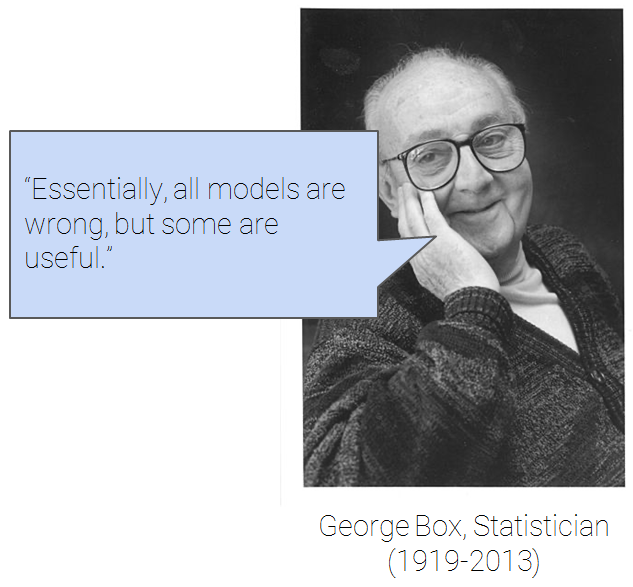
\includegraphics[scale=.4]{Bild2}
	                %\end{center}
	        \end{column}
	    \end{columns}
	\end{frame}
	
	
	
	\begin{frame}{Why do we build models?}
	    \begin{columns}
	        \begin{column}{.5\textwidth}
	                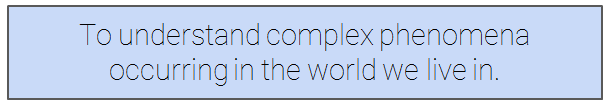
\includegraphics[scale=.4]{Bild4}
	                \begin{itemize}
	                    \item What factors play a role in the growth of COVID-19?
	                    \item How do an object’s velocity and acceleration impact how far it travels? (Physics: $d = d_0+vt+\frac{1}{2}at^2$)
	                \end{itemize}
	                Often times, we care about creating models that are simple and interpretable, allowing us to understand what the relationships between our variables are.
	                
	        \end{column}
	        
	        
	        \begin{column}{.5\textwidth}
	                    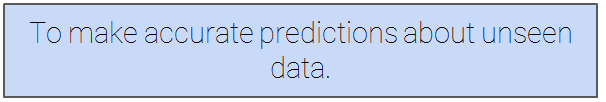
\includegraphics[scale=.4]{Bild5}
                    \begin{itemize}
	                    \item Can we predict if this email is spam or not? (Project 2!)
	                    \item Can we generate a one-sentence summary of this 10-page long article?  
	                \end{itemize}
	                Other times, we care more about making extremely accurate predictions, at the cost of having an uninterpretable model. These are sometimes called black-box models, and are common in fields like deep learning.
	        \end{column}
	    \end{columns}
	    \\\bigskip
	    Most of the time, we try to strike a balance between interpretability and accuracy.

	\end{frame}
	
	
	\begin{frame}{.}
        \begin{center}
            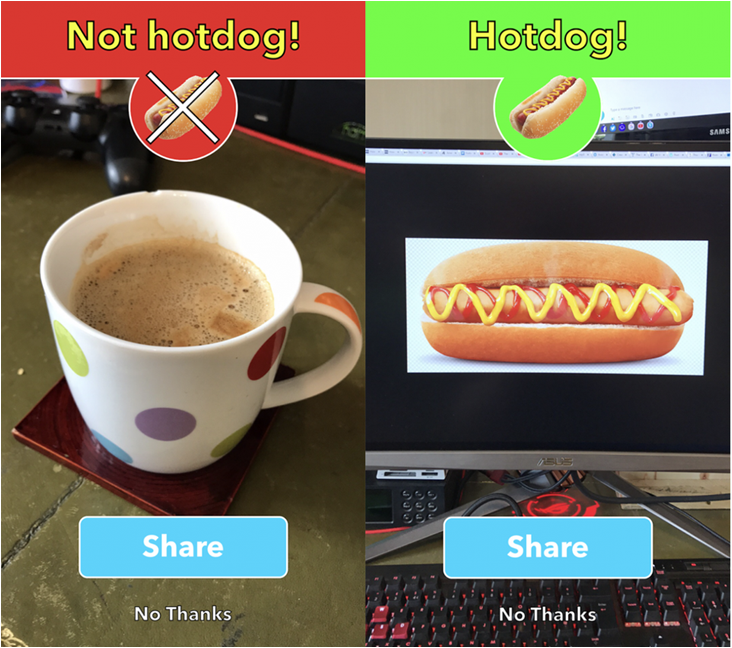
\includegraphics[scale=.5]{Bild6}
        \end{center}
	    From HBO’s Silicon Valley – hot dog or not hot dog? Behind this app is indeed a model. 
	\end{frame}
	
	
	
	\begin{frame}{Physical (or mechanistic) models}
	    Some models, such as the aforementioned model of the acceleration due to gravity on Earth, are laws that govern how the world works. We call these physical models.\\
	    \bigskip
	    \begin{columns}
	        \begin{column}{.5\textwidth}
	                Kepler's Third Law of Planetary Motion (1619)\\
	                \hspace{1cm}     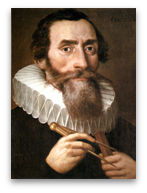
\includegraphics[scale=.5]{Bild8} \\  
	                \vspace{-1.3cm}  
	                \hspace{2.5cm} $T^2 \propto R^3$\\
	                \vspace{1.1cm}
	                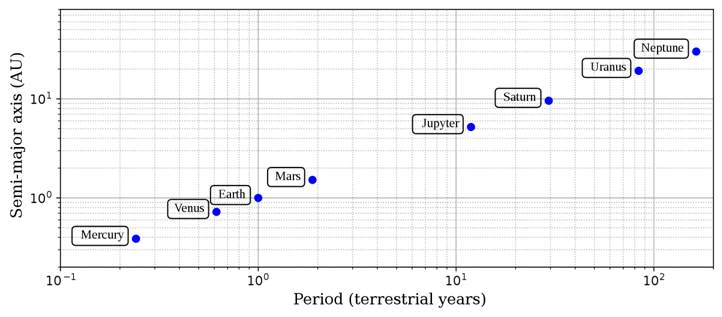
\includegraphics[scale=.5]{Bild9}
	        \end{column}
	        
	        
	        
	        \begin{column}{.5\textwidth}
	             Newton's Laws: motion and gravitation (1687)\\
                 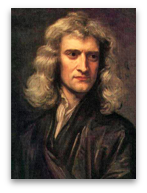
\includegraphics[scale=.5]{Bild11}\\
                 \vspace{-1.5cm}
                 \hspace{2cm}   F = ma \\
                 \hspace{2cm}   $F= G\frac{m_1m_2}{r^2}$ \\
                 \vspace{1cm}
                 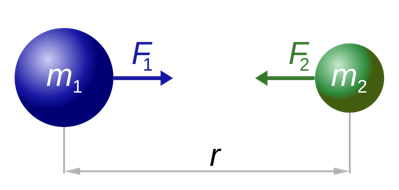
\includegraphics[scale=.7]{Bild10}
	        \end{column}
	    \end{columns}
	\end{frame}
	
	
	
	\begin{frame}{.}
	    \centering
	    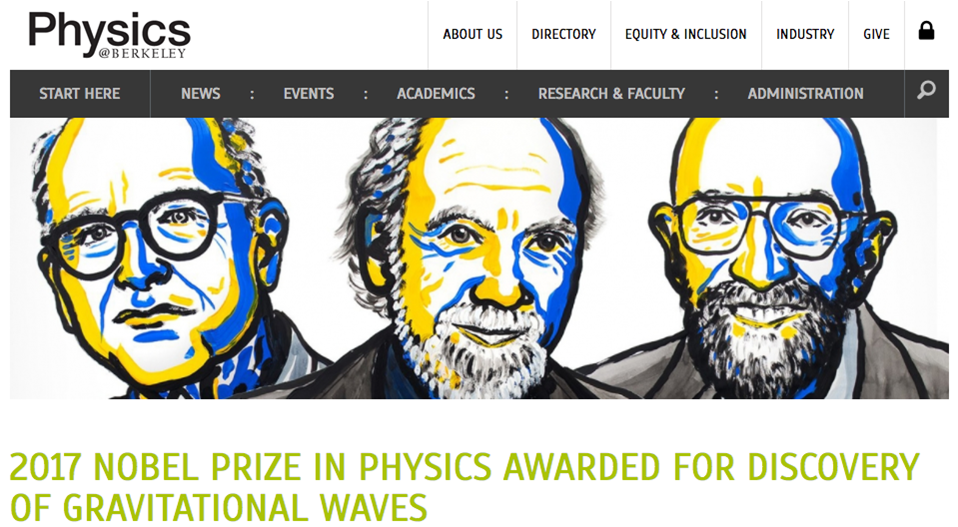
\includegraphics[scale=.55]{Bild7}
	\end{frame}
	
	
	\begin{frame}{A long time ago in a galaxy far, far away…}
	    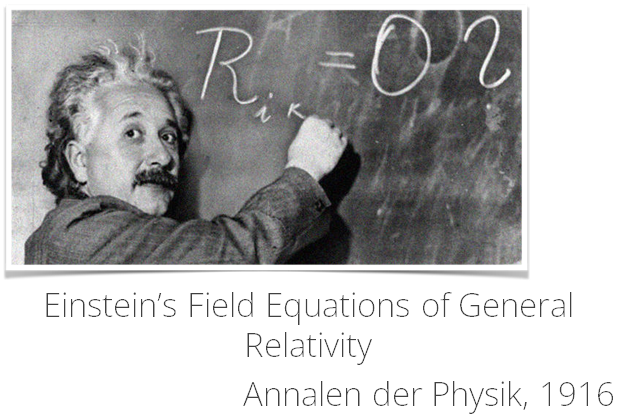
\includegraphics[scale=.5]{Bild12}\\
	    \vspace{-5cm} 
	    \hspace{8cm} $R_{\mu v} - \frac{1}{2}Rg_{\mu v} + \Lambda g_{\mu v} = \frac{8\pi G}{c^4}T\mu v$\\
	    \vspace{1cm}
	    \hspace{8.5cm}
	    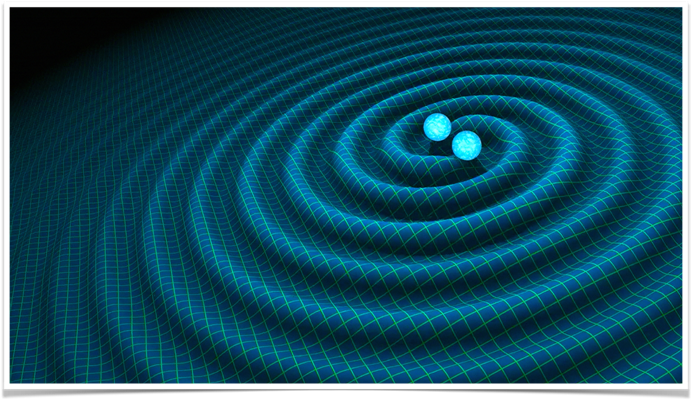
\includegraphics[scale=.5]{Bild13}
	\end{frame}
	
	
	
	\begin{frame}{.}
	    \centering
	    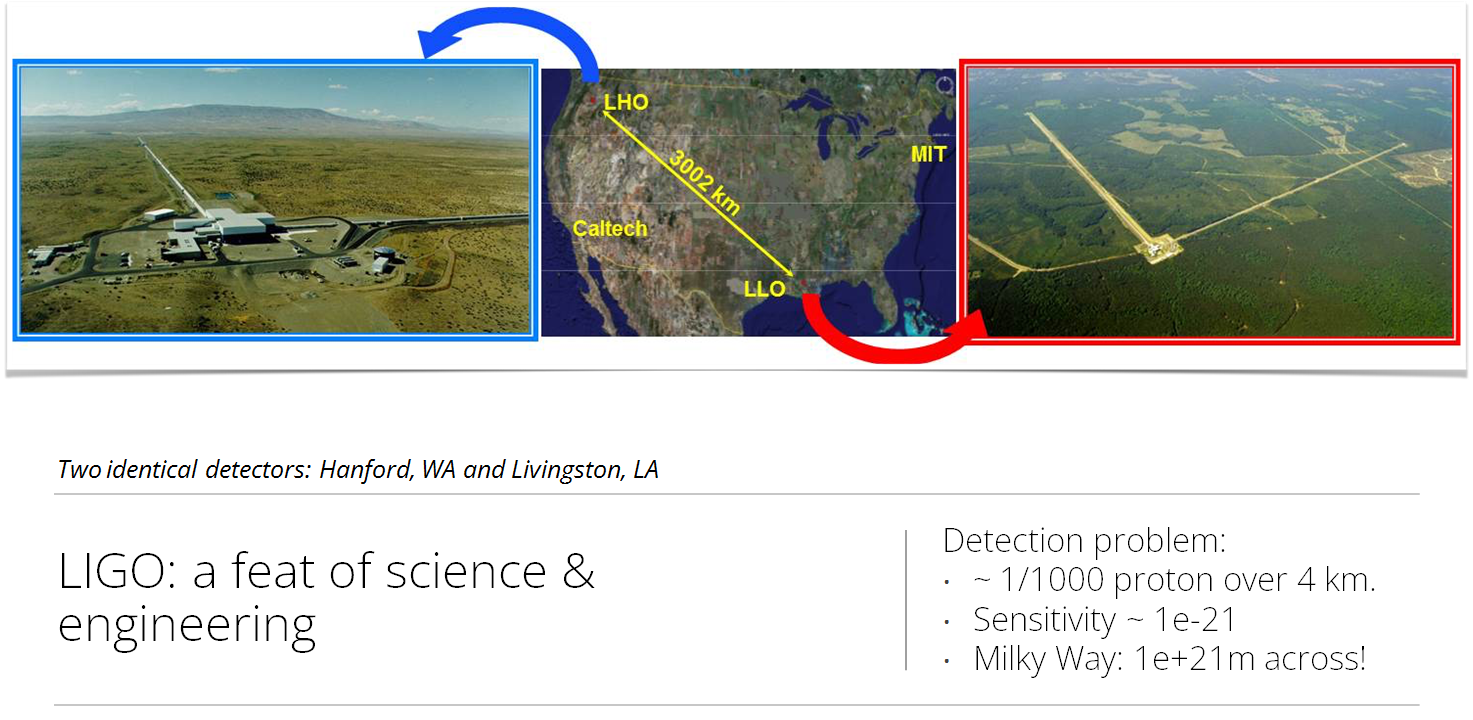
\includegraphics[scale=.35]{Bild14}
	\end{frame}
	
	
	\begin{frame}{Black holes! LIGO, Sept 14, 2015}
	    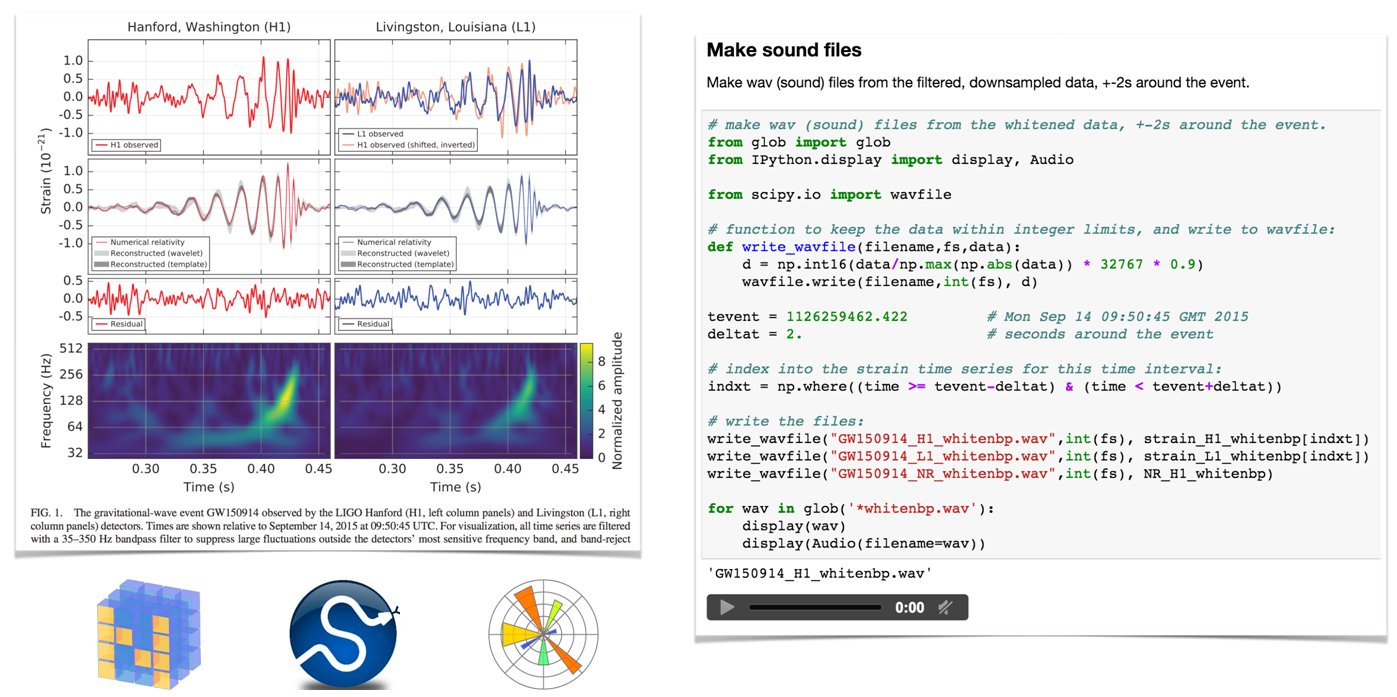
\includegraphics[scale=.35]{Bild15}\\
	    \vspace{-.5cm}
	    \hspace{7cm}  \url{http://bit.ly/black-holes-woop}
	\end{frame}
	
	
	
	\begin{frame}{Statistical models}
	    Other times, we don’t have such a precise understanding of some natural relationship. In such cases, we collect data and use statistical tools to learn more about the relationships between variables.\\
	    \hspace{1cm}
	    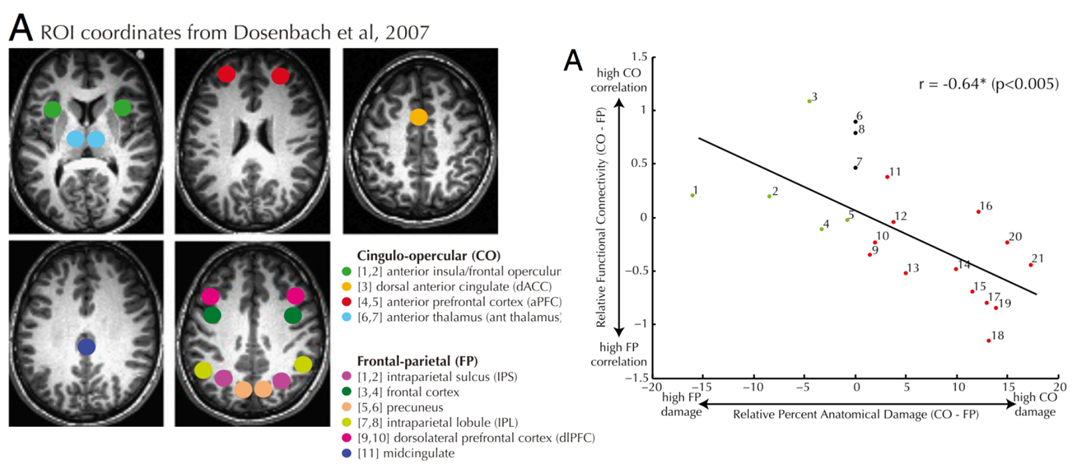
\includegraphics[scale=.45]{Bild16}
	\end{frame}
\end{document}